\documentclass[crop,tikz]{standalone}
\usetikzlibrary{shapes}
\usetikzlibrary{arrows}
\usetikzlibrary{positioning}

\begin{document}
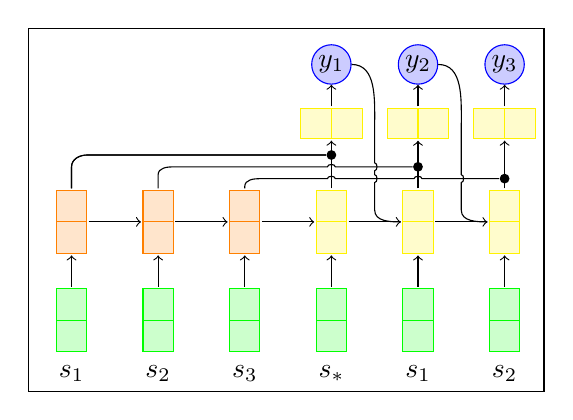
\begin{tikzpicture}[
  hid/.style 2 args={
    rectangle split,
    draw=#2,
    rectangle split parts=#1,
    fill=#2!20,
    outer sep=.25mm},
  mlp/.style 2 args={
    rectangle split,
    rectangle split horizontal,
    draw=#2,
    rectangle split parts=#1,
    fill=#2!20,
    outer sep=.25mm}
]

 % Comment out this line to remove border.
 \draw[draw=black] (-2.75, 4.21) rectangle (3.8, -.4);

 \foreach \step in {1,...,3} {
   \node (ie\step) at (1.1*\step - 3.3, -.18) {$s_\step$};
   \node[hid={2}{green}] (se\step) at (1.1*\step - 3.3, .5) {};    
   \node[hid={2}{orange}] (he\step) at (1.1 *\step - 3.3, 1.75) {};    
   \draw[->] (se\step.north) -> (he\step.south);
 } 

 \foreach \i [count=\step from 1] in {$s_*$, $s_1$, $s_2$} {
   \node (id\step) at (1.1*\step, -.18) {\i};
   \node[hid={2}{green}] (sd\step) at (1.1*\step, .5) {};    
  
   \node[hid={2}{yellow}] (hd\step) at (1.1 *\step, 1.75) {};    
   \draw[->] (sd\step.north) -> (hd\step.south);

   \node[mlp={2}{yellow}] (g\step) at (1.1 *\step, 3.0) {};    
   \node[circle, draw=blue, fill=blue!20,minimum size=5mm] (y\step) 
       at (1.1 *\step, 3.75) {};
   \node at (1.1 *\step, 3.75) {$y_\step$};    
   \draw[->] (g\step.north) -> (y\step.south);
   \draw[->] (hd\step.north) -> (g\step.south);
 }

 \node[circle,fill,inner sep=1.25pt] (t1) at (1.1 * 1, 2.60) {};
 \node[circle,fill,inner sep=1.25pt] (t2) at (1.1 * 2, 2.45) {};
 \node (t12) at (1.1 * 1, 2.45) {};
 \node[circle,fill,inner sep=1.25pt] (t3) at (1.1 * 3, 2.3) {};
% \node (t13) at (1.1 * 1, 2.40) {};
 \draw[-] (he1.north) to (1.1 - 3.3, 2.45) 
    to [out=90,in=180] (1.1 - 3.3 + .2, 2.6) to (t1.west);
 
 \draw[-] (he1.north) to (1.1 - 3.3, 2.45) 
    to [out=90,in=180] (1.1 - 3.3 + .2, 2.6) to (t1.west);
    \draw[-] (he2.north) to (2.2 - 3.3, 2.35) 
    to [out=90,in=180] (2.2 - 3.3 + .2, 2.45)
    to (1.05, 2.45) to [out=90,in=90] (1.15, 2.45) to (t2.west);
    \draw[-] (he3.north) to (3.3 - 3.3, 2.2) 
    to [out=90,in=180] (3.3 - 3.3 + .2, 2.3)
    to (1.05, 2.3) to [out=90,in=90] (1.15, 2.3) 
    to (2.15, 2.3) to [out=90,in=90] (2.25, 2.3) to (t3.west);
    
   % [out=75,in=180] (t12.center);
% \draw[-] (he3.north) to [out=90,in=180] (t13.center);
% \draw[-] (t12.center) to (t2.west);
 %\draw[-] (t13.center) to (t3.west);

 \draw[-] (y1.east) to [out=0,in=90] (1.65, 3) to (1.65, 2.50)
 to [out=0,in=0] (1.65, 2.40)
 to (1.65, 2.35) to [out=0,in=0] (1.65,2.25)
 to (1.65, 1.9) to [out=270,in=180] (hd2.west);
 
 \draw[-] (y2.east) to [out=0,in=90] (2.75, 3) to (2.75, 2.35)
 to [out=0,in=0] (2.75, 2.25) to (2.75, 1.9) to [out=270,in=180] (hd3.west);

 \foreach \last/\next in {1/2, 2/3} {
   \draw[->] (he\last.east) -> (he\next.west);
   \draw[->] (hd\last.east) -> (hd\next.west);
 }
 \draw[->] (he3.east) -> (hd1.west);


\end{tikzpicture}
\end{document}
